%%%%%%%%%%%%%%%%%%%%%%%%%%%%%%%%%%%%%%%%%%%%%%%%%%%%%
%                                                   %
%     Penn State Colloquium Poster Template         %
%                                                   %
% Uses Penn State Colloquium class, with options:   %
%                                                   %
% Orientation:                                      %
%     portrait (default), landscape                 %
%                                                   %
% Paper size:                                       %
%     a4paper (default), a0paper, a1paper, a2paper, %
%     a3paper, a5paper, a6paper                     %
%%%%%%%%%%%%%%%%%%%%%%%%%%%%%%%%%%%%%%%%%%%%%%%%%%%%%
\documentclass{../psuposter}
\renewcommand{\templateimagepath}{../} 


%%%%%%%%%%%%%%%%%%%%%%%%%%%%%%%%%%%%%%%%%%%%%%%%%%%%%
%               Package Dependencies                %
%%%%%%%%%%%%%%%%%%%%%%%%%%%%%%%%%%%%%%%%%%%%%%%%%%%%%
\usepackage{natbib}
\usepackage{lipsum}                                % Dummy text
\usepackage[figwidth = 0.98\linewidth]{todonotes}  % Dummy image (and more!)
\usepackage[absolute, overlay]{textpos}            % Figure placement
\usepackage{braket}
\setlength{\TPHorizModule}{\paperwidth}
\setlength{\TPVertModule}{\paperheight}
\setcitestyle{numbers,square}


%%%%%%%%%%%%%%%%%%%%%%%%%%%%%%%%%%%%%%%%%%%%%%%%%%%%%
%                 AUTHOR AND TITLE                  %
%%%%%%%%%%%%%%%%%%%%%%%%%%%%%%%%%%%%%%%%%%%%%%%%%%%%%
\title{Quantum Droplets and Supersolidity in a Dipolar Quantum Gas}
\author{Tilman Pfau}
\institute{University of Stuttgart}


%%%%%%%%%%%%%%%%%%%%%%%%%%%%%%%%%%%%%%%%%%%%%%%%%%%%%
%                  BEGIN DOCUMENT                   %
%%%%%%%%%%%%%%%%%%%%%%%%%%%%%%%%%%%%%%%%%%%%%%%%%%%%%
\begin{document}
\begin{frame}
\begin{columns}[t, totalwidth=\textwidth]
\begin{column}{0.45\textwidth - 1cm}


%%%%%%%%%%%%%%%%%%%%%%%%%%%%%%%%%%%%%%%%%%%%%%%%%%%%%
%                 BLOCK: BIOGRAPHY                  %
%%%%%%%%%%%%%%%%%%%%%%%%%%%%%%%%%%%%%%%%%%%%%%%%%%%%%
    \begin{block}{Speaker Biographic Summary}
    	\begin{center}
    		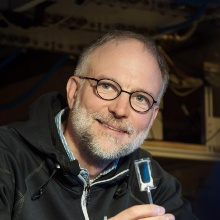
\includegraphics[width=0.6\textwidth]{images/pfau}
    	\end{center}
    	\href{https://www.uni-stuttgart.de/en/press/experts/Prof.-Tilman-Pfau/}{Dr. Tilman Pfau} is a Professor and Chair of Phototonics at the University of Stuttgart. 
    	He completed his Ph.D. in the field of atom optics at the University of Konstanz under the supervision of Prof. Jürgen Mlynek in 1994. 
    	In 2000, he founded a new institute at the University of Stuttgart for the experimental study of interacting many body systems, and he is also co-director of the Center for Integrated Quantum Science and Technology (IQST) in Stuttgart and Ulm. 
%    	He has organized various large-scale outreach activities, and serves as a spokesperson for various research networks. 
    	Prof. Pfau is an elected fellow of the Optical Society, the American Physical Society, and the American Association for the Advancement of Science, he also is a member of German and European physical societies. Dr. Pfau received the 1998 Rudolf-Kaiser Award and in 2014, the Gentner-Kastler Prize of the Société Française de Physique and the German Physical Society. He also received the APS Herbert P. Broida Prize in 2017.
    \end{block}


%%%%%%%%%%%%%%%%%%%%%%%%%%%%%%%%%%%%%%%%%%%%%%%%%%%%%
%            BLOCK: RESEARCH INTERESTS              %
%%%%%%%%%%%%%%%%%%%%%%%%%%%%%%%%%%%%%%%%%%%%%%%%%%%%%
    \begin{block}{Research Interests}
        Prof. Pfau pioneered the cooling and study of dipolar quantum gases starting from the first observation of dipolar effects in a chromium condensate, to the observation of self-bound droplets of a dilute magnetic quantum liquid. He has studied the Rydberg excitation of atoms in a quantum gas, and observed the first ultralong-range Rydberg molecules, as well as investigated the exaggerated properties of this kind of molecule. 
        \begin{center}
	    	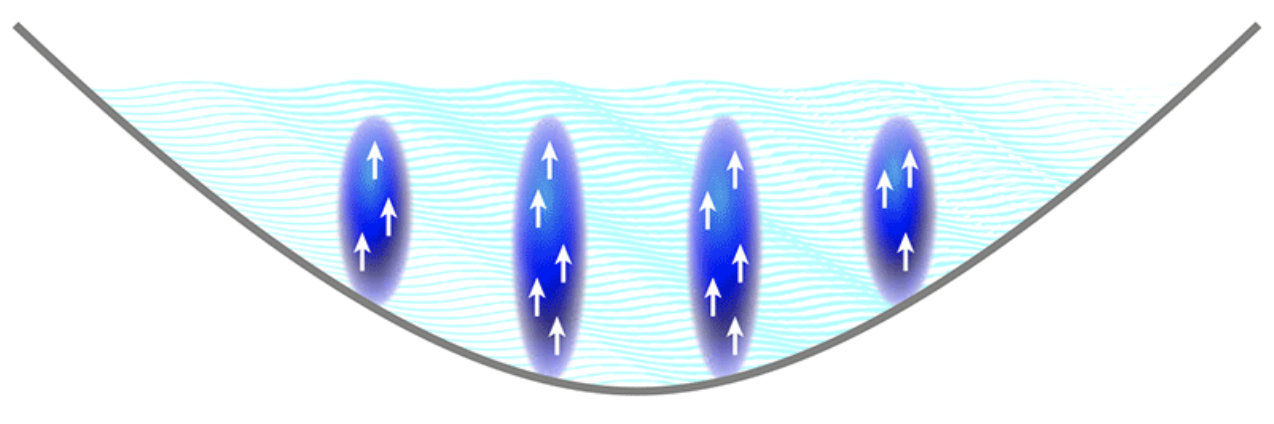
\includegraphics[width=0.95\textwidth]{images/droplet-bec}    		
    	\end{center}
    	\textit{“Droplets” form in a Bose-Einstein condensate of dipolar atoms (white arrows).} \cite{donnerDipolarQuantumGases2019}
    \end{block}
\end{column}
\begin{column}{0.55\textwidth - 1cm}


%%%%%%%%%%%%%%%%%%%%%%%%%%%%%%%%%%%%%%%%%%%%%%%%%%%%%
%                 BLOCK: ABSTRACT                   %
%%%%%%%%%%%%%%%%%%%%%%%%%%%%%%%%%%%%%%%%%%%%%%%%%%%%%
    \begin{block}{Talk Abstract}
         Dipolar interactions are fundamentally different from the usual van der Waals forces in real gases. Besides the anisotropy the dipolar interaction is nonlocal and as such allows for self organized structure formation \cite{lahayePhysicsDipolarBosonic2009a}. Similar to the Rosensweig instability in classical magnetic ferrofluids self-organized structure formation was expected. However on the meanfield level such a transition is instable due to the diluteness of the gaseous sample. In contrast to these predictions in 2015 we could observe the formation of a stable droplet crystal and found that this unexpected stability is due to beyond mean-field quantum corrections of the Lee-Huang-Yang type. When arranged in a 1D array also phase coherence between the droplets was observed, which was first evidence for a supersolid state of matter. Upon crossing the transition to the dipolar supersolid a Goldstone mode appears, which we have observed. The existence of this mode proofs the superfluid stiffness or the so-called phase rigidity of this new state of matter. Recently we have also measured the static structure factor across the transition which allows to show that the characteristic fluctuations correspond to elementary excitations such as the roton modes, and that the supersolid state supports both superfluid as well as crystal phonons. A recent review on the discovery of quantum dropets and dipolar supersolids can be found in ref. \cite{bottcherTransientSupersolidProperties2019a}.
    \end{block}


%%%%%%%%%%%%%%%%%%%%%%%%%%%%%%%%%%%%%%%%%%%%%%%%%%%%%
%                BLOCK: BACKGROUND                  %
%%%%%%%%%%%%%%%%%%%%%%%%%%%%%%%%%%%%%%%%%%%%%%%%%%%%%
    \begin{block}{Brief Background}
    Classically, the phases of matter- solid, liquid and gas are understood as an interplay between the strength of interactions and the kinetic energy of the particles. In the quantum regime, a similar interplay between the quantum fluctuations and interparticle interaction leads to yet newer phases of matter like the supersolid which features periodic density modulation of a solid together with dissipationless flow of a superfluid.  Supersolidity has since been observed in ultracold atomic systems for Bose-Einstein Condensates (BECs) configurations. \cite{lahayePhysicsDipolarBosonic2009a} 
        \begin{center}
		   	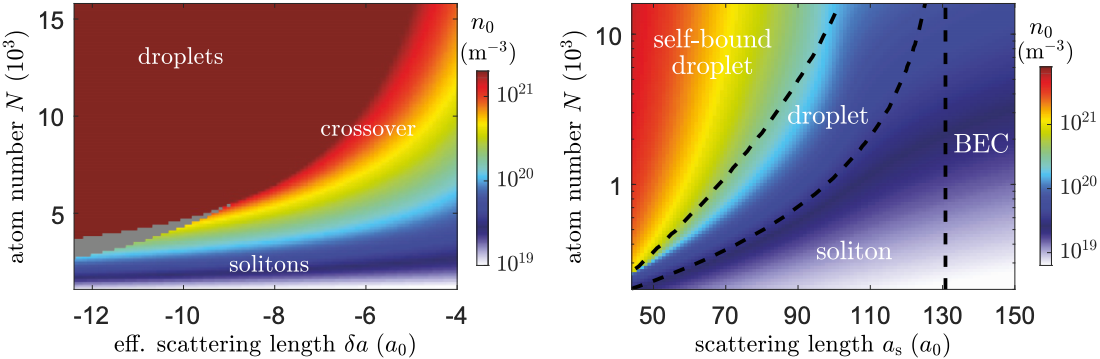
\includegraphics[width=0.75\textwidth]{images/droplet}    		
    	\end{center}
		 A new line of investigation for finding such supersolid behaviour is in dilute, dipolar quantum gases which feature both short-range contact interactions as well as long-range dipole-dipole interactions. Although once thought unstable, supersolidity has been observed in trapped dipolar gases. \cite{bottcherNewStatesMatter2020} 

    \end{block}


%%%%%%%%%%%%%%%%%%%%%%%%%%%%%%%%%%%%%%%%%%%%%%%%%%%%%
%                 BLOCK: REFERENCES                 %
%%%%%%%%%%%%%%%%%%%%%%%%%%%%%%%%%%%%%%%%%%%%%%%%%%%%%
    \begin{block}{References}
        \bibliographystyle{aipnum4-1}
%        \bibliographystyle{iopart-num}
		\bibliography{references}
    \end{block}

\end{column}
\end{columns}


%%%%%%%%%%%%%%%%%%%%%%%%%%%%%%%%%%%%%%%%%%%%%%%%%%%%%
%                    FOOTER TEXT                    %
%%%%%%%%%%%%%%%%%%%%%%%%%%%%%%%%%%%%%%%%%%%%%%%%%%%%%
\begin{textblock}{0.5}(0.18, 0.94)
    \color{white}
    \sffamily
    \textbf{Eberly College of Science}
    \\
    Department of Physics
\end{textblock}


%%%%%%%%%%%%%%%%%%%%%%%%%%%%%%%%%%%%%%%%%%%%%%%%%%%%%
%                   END TEMPLATE                    %
%%%%%%%%%%%%%%%%%%%%%%%%%%%%%%%%%%%%%%%%%%%%%%%%%%%%%
\end{frame}
\end{document}
